\section{Progress}

Where are we with design/implementation?

We have made a simple Unity project containing camera pointing at a plane that has a texture of a screenshot from Google Maps. 
We intend to use this plane as a reference for whatever location we use in the program.
See the image below:

\begin{figure}[htb]
    \centering
    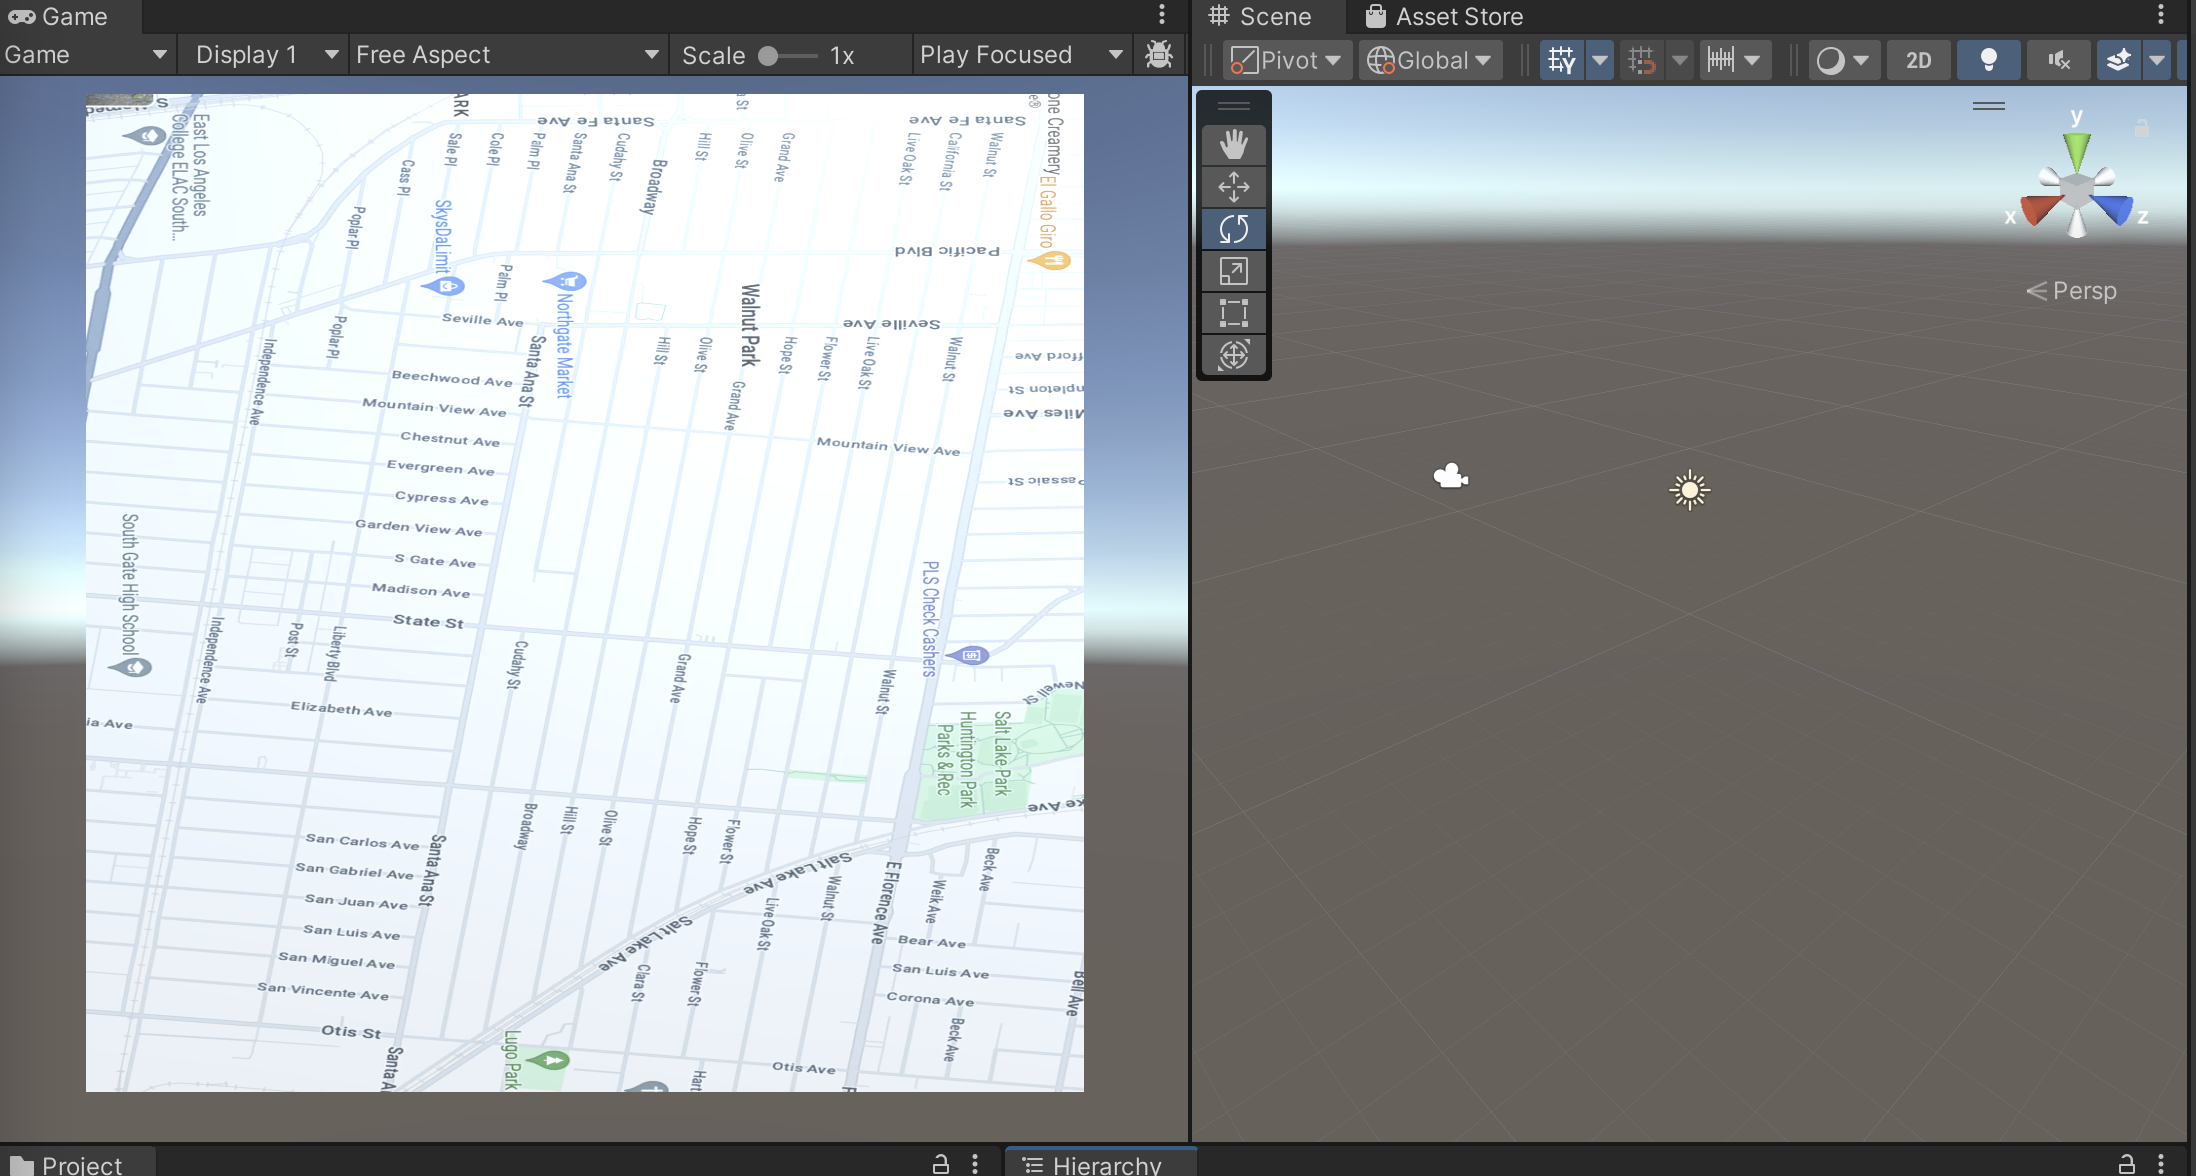
\includegraphics[width=10cm]{../Images/ProjectProgress1.png}
       \caption{Screenshot of current Unity project with Game Panel on left.}
           \label{Fig:UnityProject1}
  \end{figure}

\begin{flushleft}
We also decided on a plan for how to structure our architecture for the project moving forward. 
As seen with the diagram below, we decided on 3 levels of computation/algorithms that will happen behind the UI scene:
\begin{itemize}
    \item Where the project will ask the User for a location.
    \item Feed the given user input into a script that will connect it to a webpage.
    \item This webpage will make the map and return it back to that script.
    \item The script will return the image to the Unity project.
    \item We then run the traffic model made with Machine Learning on that map with traffic data. 
 \end{itemize}
\end{flushleft}


\begin{figure}[htb]
    \centering
    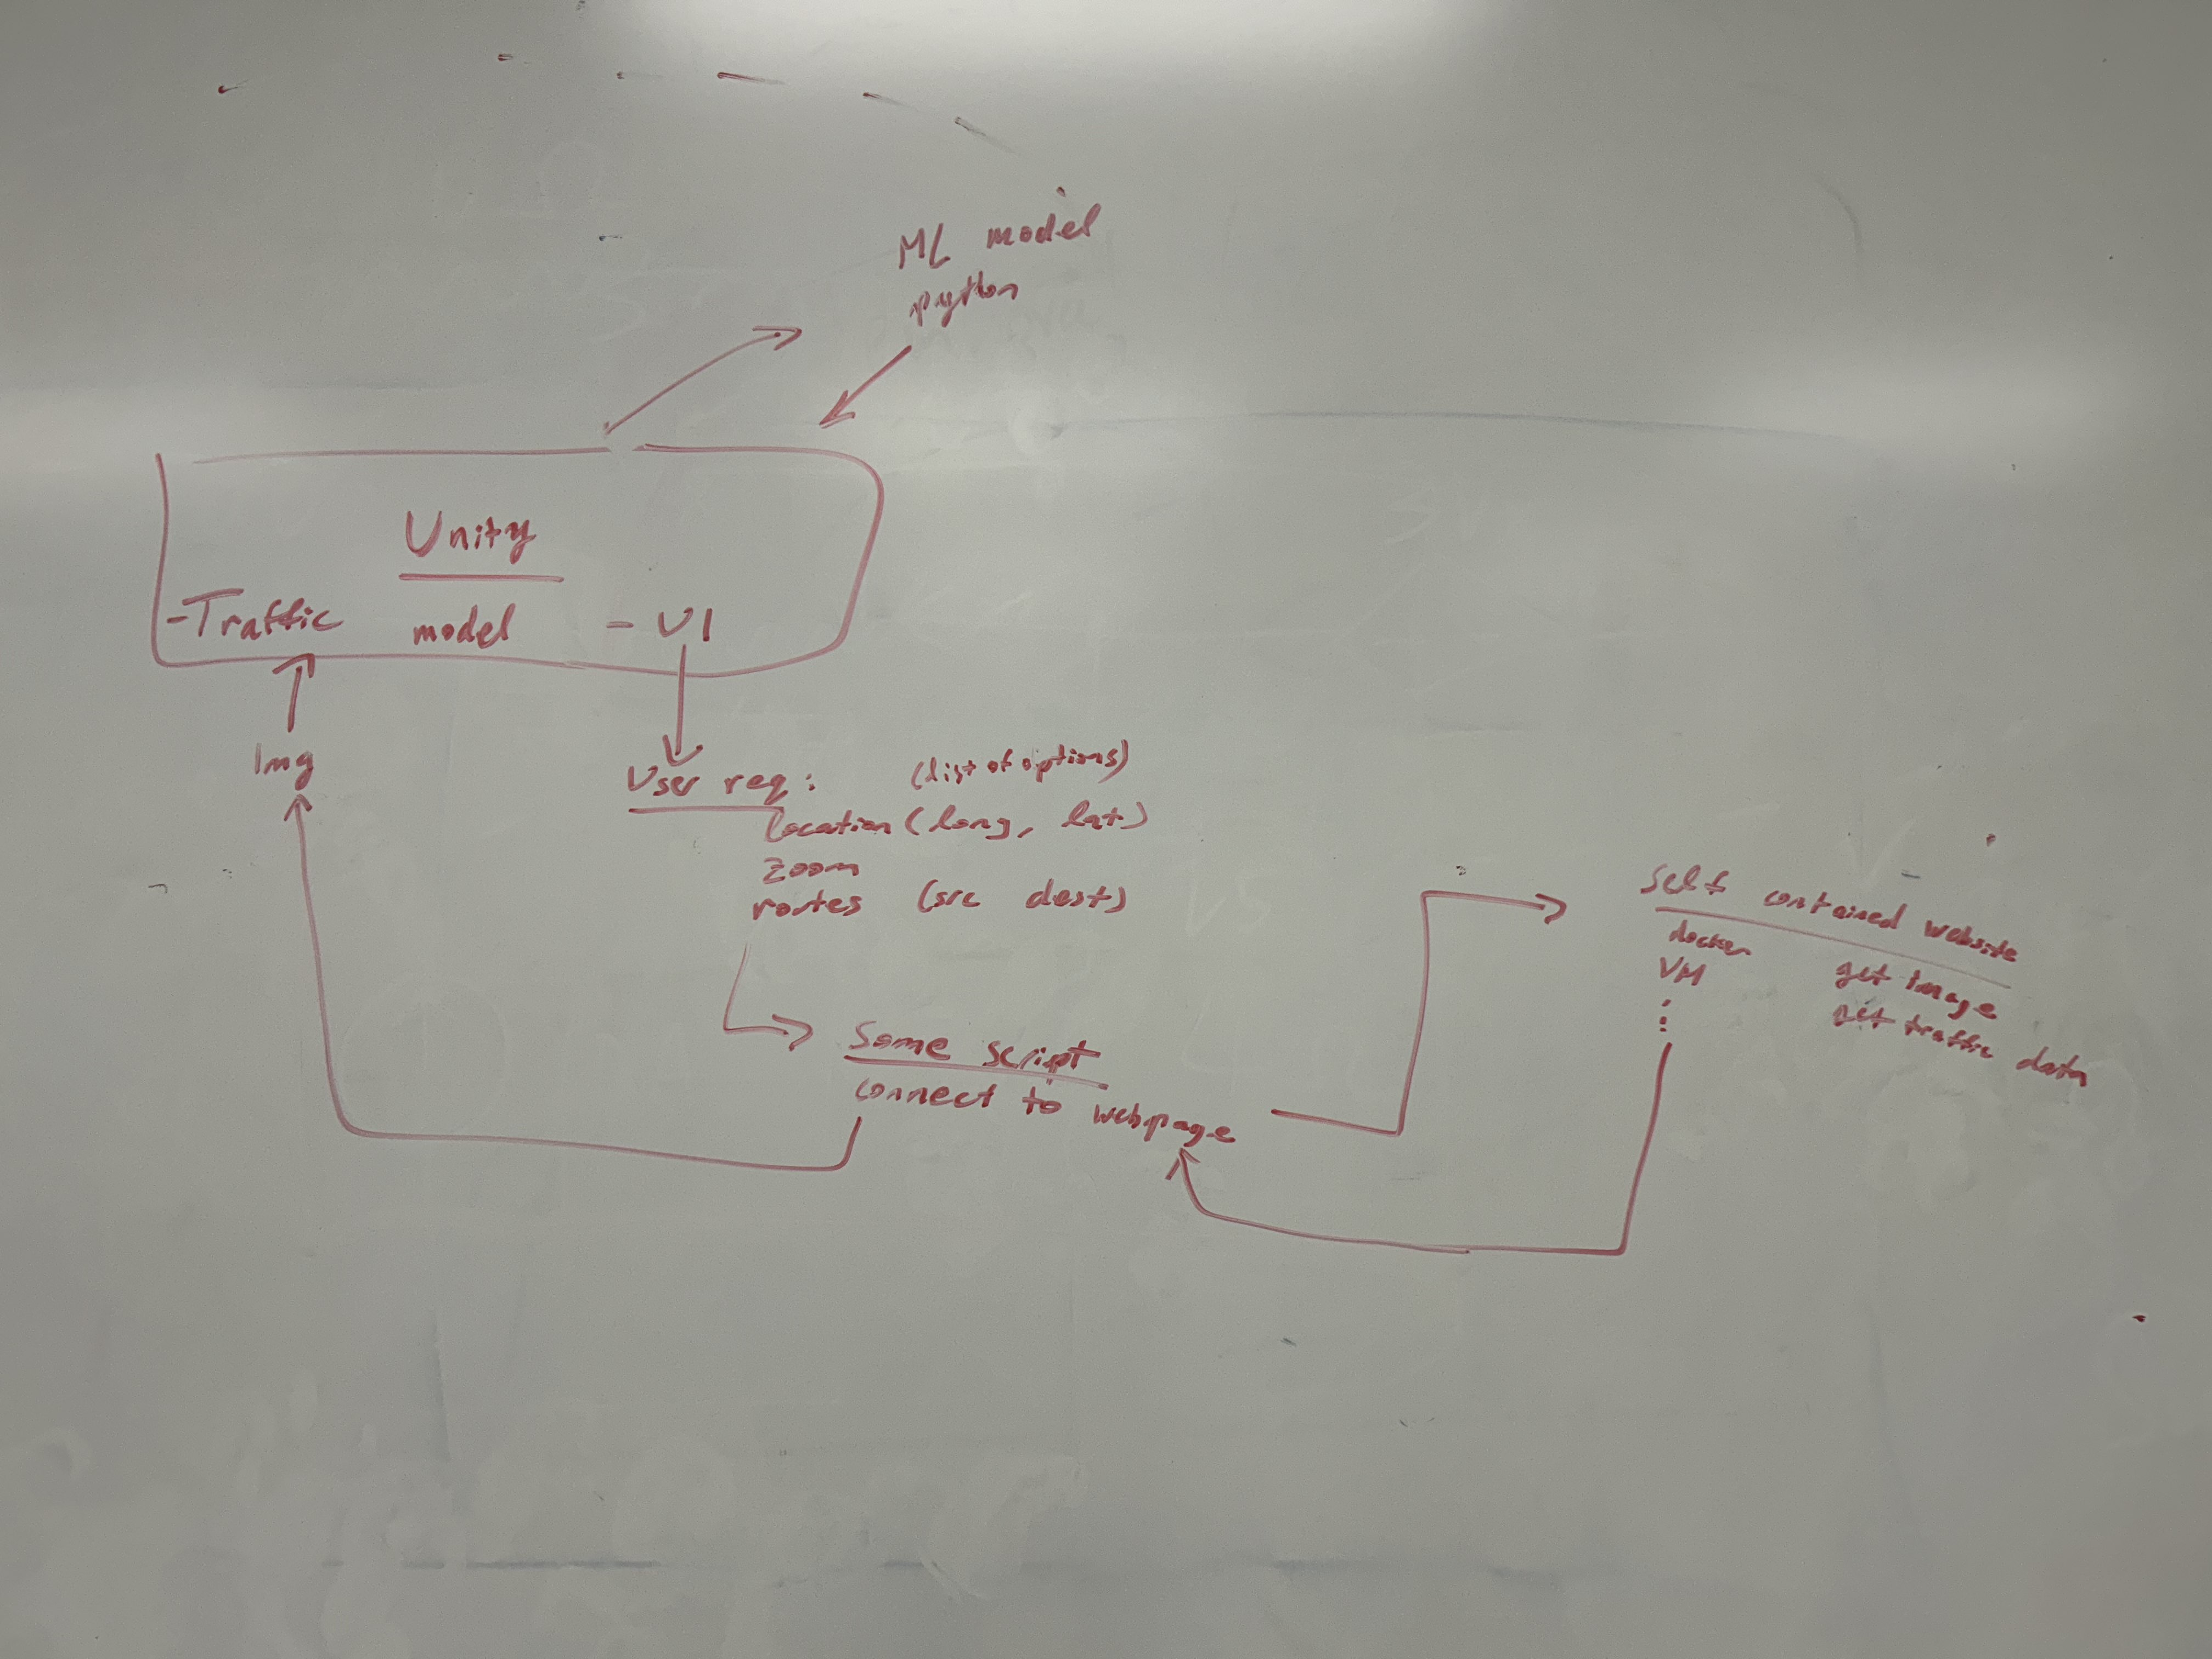
\includegraphics[width=10cm]{../Images/ArchitectureDiagram.jpg}
       \caption{Sample Architecture Diagram outlined in Class 2/19/24.}
           \label{Fig:ArchitectureDiagram}
  \end{figure}


\begin{flushleft}
Since the traffic data that we had found wasn't very consistent, one intersection would have data from 2015 when the other intersection nearby only had data from 1983.
We are currently working towards grabbing a fixed amount of data for one location rather than letting the User input any random longitude and latitude for the program to run with. 
Instead, we are thinking of presenting the user with 3 or 4 options to choose from which is our fixed set of data to run. \par

Additionally, Isaiah has set up a GitHub page for writing both our reports as well as adding any implementations and ML models for the project which can be seen in Figure \ref{Fig:GitPage}.
\end{flushleft}


\begin{figure}[htb]
    \centering
    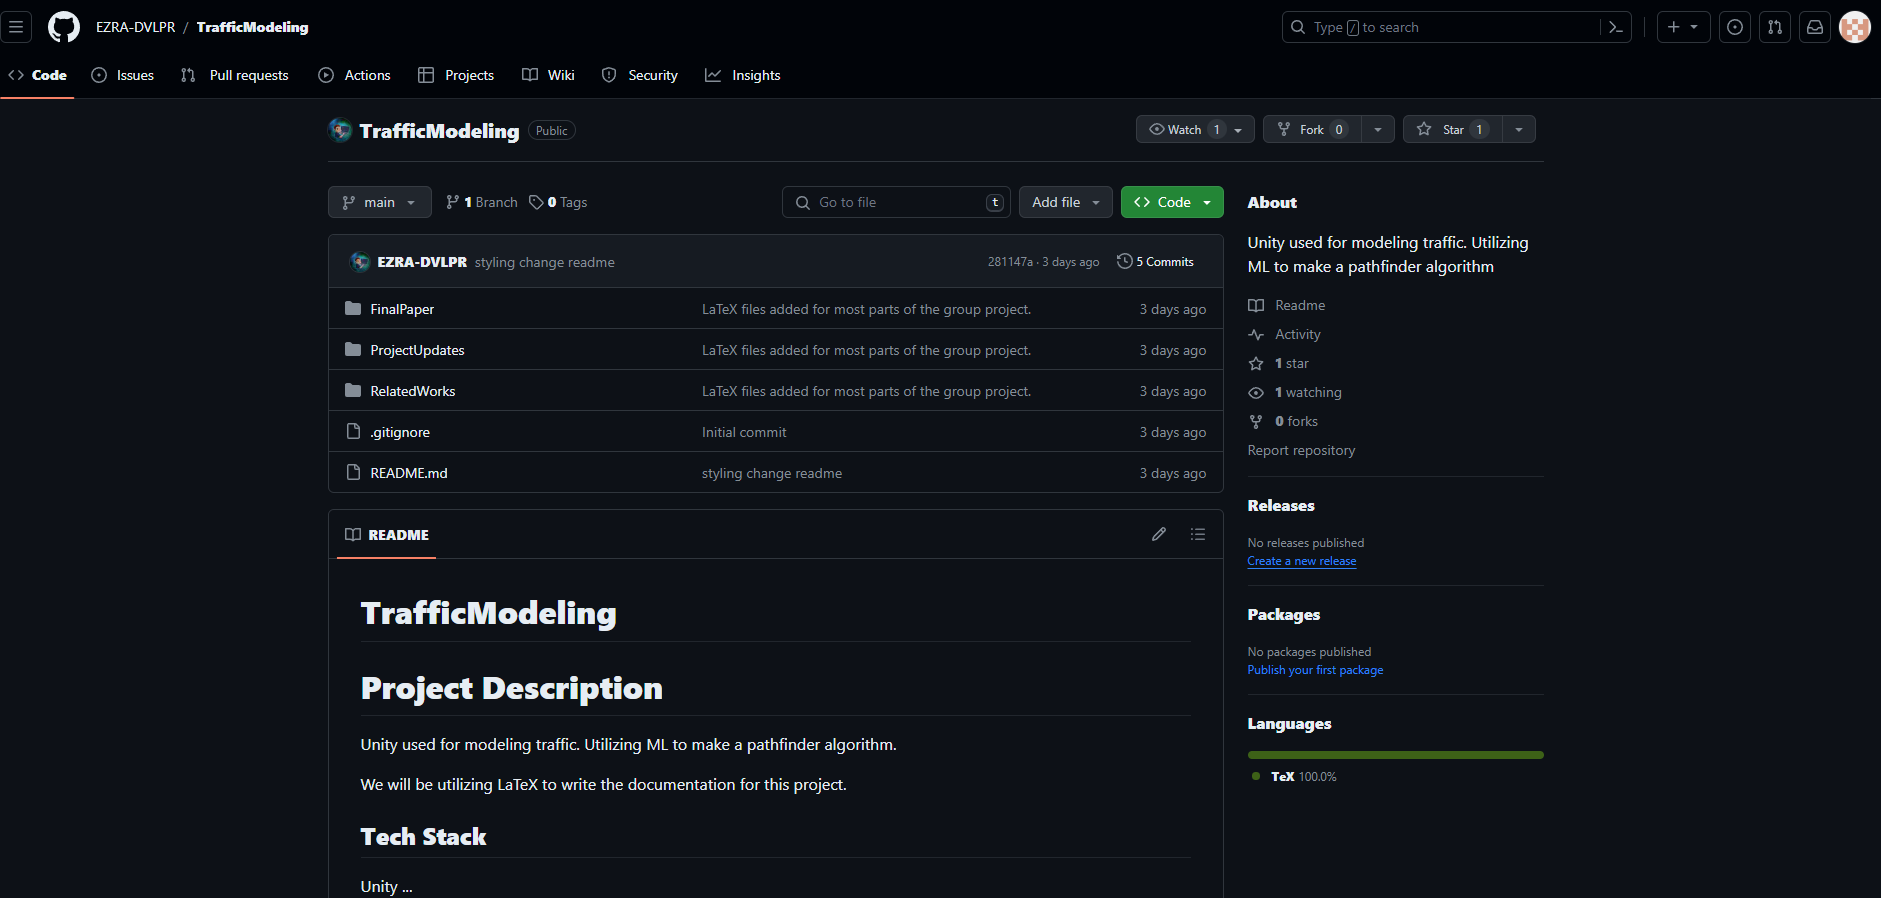
\includegraphics[width=10cm]{../Images/GitPage.png}
       \caption{Screenshot of the Git Page.}
           \label{Fig:GitPage}
\end{figure}

\newpage